\subsection{\texorpdfstring{Group Law on the Classes of \(\tau\)-Extensions}{Group Law on the Classes of \textbackslash tau-Extensions}}

Let \(\mathrm{G}\) be a group, \(\mathrm{F}\) be an abelian group, and \(\tau : \mathrm{G} \to \mathrm{Aut}(\mathrm{F})\) be a group homomorphism. We denote by \(\delta : \mathrm{G} \to \mathrm{G} \times \mathrm{G}\) the diagonal mapping \(g \mapsto (g, g)\) and by \(m : \mathrm{F} \times \mathrm{F} \to \mathrm{F}\) the multiplication homomorphism \((f_1, f_2) \mapsto f_1 f_2\) . We denote by \(s : \mathrm{F} \to \mathrm{F}\) the group homomorphism given by \(f \mapsto f^{-1}\) . Let \(\mathcal{E}_1 = (\Gamma_1, \iota_1, \pi_1)\) and \(\mathcal{E}_2 = (\Gamma_2, \iota_2, \pi_2)\) be \(\tau\) -extensions of \(\mathrm{G}\) by \(\mathrm{F}\) . Since we have the relation

\[
m (((\tau \times \tau) \circ \delta) (g) \cdot (f _ {1}, f _ {2})) = \tau (g) \cdot m (f _ {1}, f _ {2})
\]

for every \(g \in G\) and all \(f_{1}, f_{2} \in F\) , the extension \(m_{*}(\delta^{*}(\mathcal{E}_{1} \times \mathcal{E}_{2}))\) is a \(\tau\) -extension; we call it the product of the \(\tau\) -extensions \(E_{1}\) and \(E_{2}\) and denote it by \(E_{1}E_{2}\) . The class of this extension depends only on the classes of the extensions \(E_{1}\) and \(E_{2}\) (VIII, p.~288, Corollary 1 and VIII, p.~291, Corollary 1). So this gives a law of composition on \(\operatorname{Ex}_{\tau}(\mathbf{G}, \mathbf{F})\) .

Remark. --- Let \(\mathcal{E}_{1}=(\Gamma_{1},\iota_{1},\pi_{1})\) and \(\mathcal{E}_{2}=(\Gamma_{2},\iota_{2},\pi_{2})\) be \(\tau\) -extensions of G by F. Let \(\mathcal{E}_{1}\mathcal{E}_{2}=(\Gamma,\iota,\pi)\) be the product of these extensions. Following the example of VIII, p.~289, the construction gives a surjective group homomorphism from the fiber product \(\Gamma_{1}\times_{G}\Gamma_{2}\) to \(\Gamma\) whose kernel is the image of the group homomorphism \(f\mapsto(\iota_{1}(f),\iota_{2}(f)^{-1})\) from F to \(\Gamma_{1}\times_{G}\Gamma_{2}\) .

PROPOSITION 4. --- The product of \(\tau\) -extensions endows the set \(\mathrm{Ex}_{\tau}(\mathrm{G},\mathrm{F})\) with the structure of an abelian group. Its identity element is the class of the semitrivial extension \(\mathcal{I}_{\tau}\) . The inverse of the class of a \(\tau\) -extension \(\mathcal{E}\) is the class of \(s_{*}(\mathcal{E})\) .

The associativity of the law follows from the commutativity of the diagrams

\pandocbounded{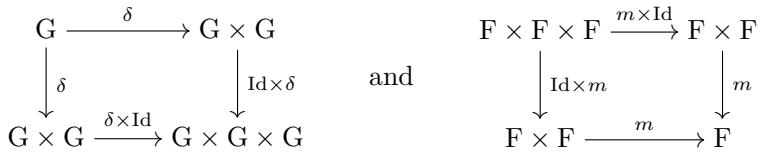
\includegraphics[keepaspectratio]{images/part002_39f17f00.jpg}}

and from Corollary 2 of VIII, p.~288; Corollary 2 of VIII, p.~291; and Proposition 3 of VIII, p.~292.

Let \(\Delta : \mathrm{F} \to \mathrm{F} \times \mathrm{F}\) be the diagonal mapping \(f \mapsto (f, f)\) . Let \(\mathcal{E} = (\Gamma, \iota, \pi)\) be a \(\tau\) -extension. Let \(\widetilde{\Delta}: \Gamma \to \Gamma \times_{\mathrm{G}} \Gamma\) be the group homomorphism given by \(\gamma \mapsto (\gamma, \gamma)\) . The following diagram commutes:

\pandocbounded{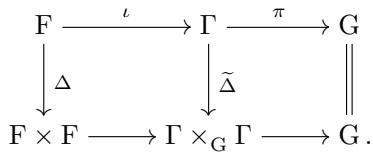
\includegraphics[keepaspectratio]{images/part002_db57599b.jpg}}

By Proposition 2 of VIII, p.~290, it follows that the \((\tau \times \tau) \circ \delta\) -extension \(\delta^{*}(\mathcal{E} \times \mathcal{E})\) is isomorphic to \(\Delta_{*}(\mathcal{E})\) .

Denote by \(c: F \to F\) the constant homomorphism \(f \mapsto 1\) . by Example 1 of VIII, p.~292, the fact that \(\mathcal{I}_{\tau}\) is an identity element for this law of composition follows from the isomorphism from \(\delta^{*}(\mathcal{E} \times \mathcal{E})\) to \(\Delta_{*}(\mathcal{E})\) and the commutative diagram

\pandocbounded{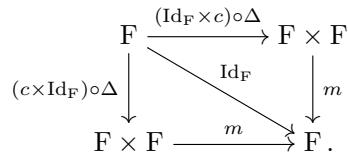
\includegraphics[keepaspectratio]{images/part002_761b87f2.jpg}}

The last assertion follows from the commutative diagram

\[
\begin{array}{c} \mathrm{F} \xrightarrow {(\mathrm{Id} _ {\mathrm{F}} \times s) \circ \Delta} \mathrm{F} \times \mathrm{F} \\ (s \times \mathrm{Id} _ {\mathrm{F}}) \circ \Delta \Biggl \downarrow \qquad \qquad \qquad \qquad \qquad \qquad \qquad \qquad \qquad \qquad \qquad \qquad \qquad \qquad \qquad \qquad \qquad \qquad \qquad \qquad \qquad \qquad \qquad \qquad \qquad \qquad \qquad \qquad \qquad \qquad \qquad \qquad \qquad \qquad \\ \mathrm{F} \times \mathrm{F} \xrightarrow {m} \mathrm{F}. \end{array}
\]

Let \(\mathcal{E}_1 = (\Gamma_1,\iota_1,\pi_1)\) and \(\mathcal{E}_2 = (\Gamma_2,\iota_2,\pi_2)\) be \(\tau\) -extensions. The group isomorphism \(\Gamma_1\times \Gamma_2\to \Gamma_2\times \Gamma_1\) given by \((\gamma_{1},\gamma_{2})\mapsto (\gamma_{2},\gamma_{1})\) restricts to a group isomorphism \(\sigma :\Gamma_1\times_\mathrm{G}\Gamma_2\to \Gamma_2\times_\mathrm{G}\Gamma_1\) . Because of the relations

\[
\sigma (\iota_ {1} (f), \iota_ {2} (f) ^ {- 1}) = (\iota_ {2} (f ^ {- 1}), \iota_ {1} (f ^ {- 1}) ^ {- 1})
\]

for \(f \in F\) , the group homomorphism \(\sigma\) induces, by passing to the quotients, a morphism of \(\tau\) -extensions from \(E_{1}E_{2}\) to \(E_{2}E_{1}\) . So the law of composition is commutative.

PROPOSITION 5. --- a) Let G and G' be groups, and let F be an abelian group. Let \(\tau: \mathrm{G} \to \operatorname{Aut}(\mathrm{F})\) and \(u: \mathrm{G}' \to \mathrm{G}\) be group homomorphisms. The mapping \(u^*: \operatorname{Ex}_{\tau}(\mathrm{G}, \mathrm{F}) \to \operatorname{Ex}_{\tau \circ u}(\mathrm{G}', \mathrm{F})\) is a group homomorphism.

\begin{enumerate}
\def\labelenumi{\alph{enumi})}
\setcounter{enumi}{1}
\tightlist
\item
  Let G be a group, and let F and \(F'\) be abelian groups. Let \(\tau: G \to \text{Aut}(F)\) , \(\tau': G \to \text{Aut}(F')\) , and \(v: F \to F'\) be group homomorphisms such that
\end{enumerate}

\[
\tau^ {\prime} (g) \cdot v (f) = v (\tau (g) \cdot f)
\]

for \(g \in \mathrm{G}\) and \(f \in \mathrm{F}\) . The mapping \(v_{*} : \operatorname{Ex}_{\tau}(\mathrm{G}, \mathrm{F}) \to \operatorname{Ex}_{\tau'}(\mathrm{G}, \mathrm{F}')\) is a group homomorphism.

This follows from the commutativity of the diagrams

\[
\begin{array}{l} \mathrm{G} ^ {\prime} \xrightarrow {\delta} \mathrm{G} ^ {\prime} \times \mathrm{G} ^ {\prime} \\ \Biggl \downarrow_ {u} \qquad \Biggl \downarrow_ {u \times u} \\ \mathrm{G} \xrightarrow {\delta} \mathrm{G} \times \mathrm{G} \end{array} \qquad \text {and} \qquad \begin{array}{l} \mathrm{F} \times \mathrm{F} \xrightarrow {m} \mathrm{F} \\ \Biggl \downarrow_ {v \times v} \qquad \Biggl \downarrow_ {v} \\ \mathrm{F} ^ {\prime} \times \mathrm{F} ^ {\prime} \xrightarrow {m} \mathrm{F} ^ {\prime}. \end{array}
\]

